\documentclass[a4paper,12pt]{article}
\usepackage[margin=0.7in]{geometry}
\usepackage[latin1]{inputenc}
\usepackage[english]{babel}
\usepackage{amsmath}
\usepackage{cases}
\usepackage[makeroom]{cancel}
\usepackage{amsmath,tabu}
\usepackage[fleqn]{mathtools}
\usepackage[fleqn]{amsmath}
\usepackage{bm}
\usepackage{tikz}
\usepackage{enumitem}
\usepackage{wrapfig}
\usepackage{graphicx}
\usepackage{siunitx}
\usepackage{microtype}
\usepackage{array,tabularx}
\usepackage{float}
\usepackage{booktabs}
\usepackage{import}
\usepackage{cases}
\usepackage{graphicx,subfigure}
\usepackage{myUnitOfMeasure}
%\usepackage{myThermodynamics}
\usepackage{myMath}
\usepackage{mathtools}
\usepackage{gensymb}
\usepackage{xcolor}
\usepackage{url}
\usepackage{tabularx}
\usepackage{ltablex}

\title{

\includegraphics[scale=0.4]{images/logo.png}
\\[1cm]
FINAL REPORT ON THE  MRL TURBINE SIMULATION
COURSE OF MODELING TECHNIQUES FOR FLUID MACHINES 
A.Y. 2017/2018}
\author{
Andrea Rossi \and Marco Bonasegale
\and Marco Belloli \and Alberto Casali 
}
\date{}

% usefull for ltablex to split long tables in many pages
\keepXColumns

\DeclarePairedDelimiter\abs{\lvert}{\rvert}%

%\newcommand{\Fy}[1]{\text{F}_{y_{#1}}}

%\newcommand{\diameter}{\oslash}

%\newcommand{\todo}{\colorbox{cyan!60}{TODO}}

\renewcommand{\thesubsection}{\thesection.\arabic{subsection}}

\renewcommand{\arraystretch}{1.4}

\newcommand{\variable}[1]{\textcolor{blue}{#1}}

\newcommand{\paramtext}[1]{\textcolor{black!30!green}{#1}}

\newcommand{\terminal}[1]{\textcolor{black!30!cyan}{#1}}

\newcommand{\todo}{\colorbox{cyan!60}{TODO}}

\makeindex

\begin{document}



\maketitle

\newpage

\tableofcontents

\newpage

\section{Introduction}

\subsection{MRL Tidal Turbine Description}
The MRL Turbine is a hydraulic machine which is able to exploit the upcoming  water flow that is passing through the cross sectional area of the inlet of the machine. Momentum Reversal and Lift Tidal Turbine is a cross-
flow tidal-stream device which converts
 the energy of the water
flow into mechanical power.So the most advantageous locations in order to place this device are whatever kind of regular river with a smooth river bed or any sea/ocean areas which are subjected to relevant tidal phenomena.
The turbine is made up of three rotating blades and each blade is subjected to the combination of two rotating motions. A rotation $\omega_0$ along the machine axis  and a rotation omega1 around the blade individual axis with counter-rotating $\omega_0$ and $\omega_1$.

\begin{center}
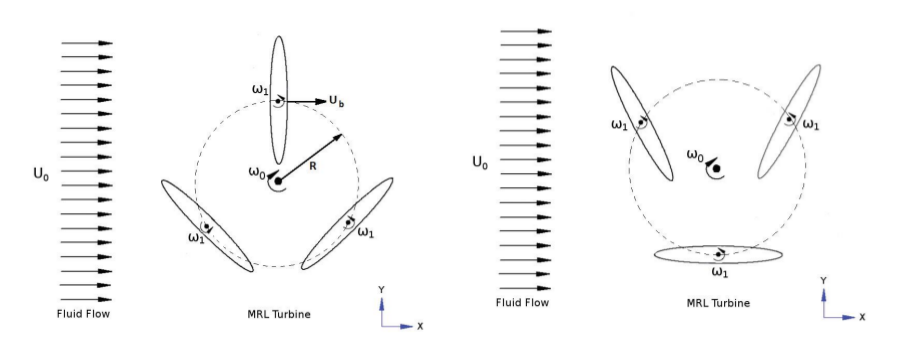
\includegraphics[width=0.8\textwidth]{images/flow.png} 
\end{center}

The flow-blade interaction leads to a drag force that is coming out while the blade is placed in the upper part of the circumferential path and a lift force on each blade located in the lower part of the path.
The resulting torque multplied by the rotating speed will give the generated power of the turbine which, in the end, is our final useful effect. The generated power per turbine is not really high (a few Watts) and this is the reason why the \emph{farm layout}  that Prof. Gavin Tabor showed us at the beginning of the course is used. Many little turbines are placed in a schematic and regular disposition in order to extract a higher power from the tidal stream.
Since from the first raw presentation of the machine we can realise that the mesh will have a relevant importance in the representation and validation of this complex rotating movement. We will deal with a rotating mesh which is progressivly refined closeto the blades, ending with the boundary layers when we are approaching the solid walls of the blades.


\subsection{The data}
The turbine is surrounded by an upcoming water flow set at 1 m/s constant along y axis. 
CAD files were provided by our professor and all the geometry parameters were known.
The in-class workflow has been divided into four little sub-tasks. 

The sub-tasks allowed us to start to get more familiar with the project work and understand the main issues met along the path with the help of the professors. The in-class project started with the raw mesh generation (blockMesh, snappyHexMesh), continued with the preparation of the rotating mesh(AMI files, baffles creation, merge and split procedure), movement of the mesh with the provided motion laws  (real turbine rotation, gif rendering) and finally the set up, running and post processing of the simulation.

\section{Mesh sensitivity Analysis}


\section{Numerical Schemes}

\section{Gravitational influence}

\section{Turbolence}

\subsection{Turbolence model}

\paragraph{Laminar}

\paragraph{$k-\varepsilon$ model}

\paragraph{$k-\omega $ SST model}

\subsection{Turbolence intensity}

\section{The domain's sizes}

\section{Results}

\section{Blade speed ratio Analysis}

From what we have seen in mesh sensitivity analysis, the power is quite accurately computed even for a mesh size smaller that that we consider mesh independent.

To obtain a larger number of points from the blade speed ratio analysis we have decided to run most of the simulation with a mesh with 80 cells in the y direction instead of 120. This reduces the number of cells to around 60000 instead of 110000. 
\\Computational time is in this way reduced, but we are not sure that the result is correct.

So we validate just the most significant points with the finer mesh and we compare with the results of the coarser.

We consider that this operating procedure is a proper balance between accuracy and computational cost.

\todo{include fig}

As the mesh sensitivity analysis already highlighted, power is not influenced to much even with this coarser mesh and the difference with the finer mesh is almost negligible.

\subsection{Comparison with experiments}

The trends highlighted by our CFD simulation follow quite accurately that from the real experiments.
The main difference is in terms of absolute value of the power computed. 
This can highlight a difference between the simulated case and the real one, in terms of solidity, ecc \todo 

\section{Conclusion}


















\end{document}